
\documentclass{article}

\usepackage[pdftex]{graphicx}
	\graphicspath{{../figures/}}
	\DeclareGraphicsExtensions{.pdf,.jpeg,.png}
\usepackage{amsmath}
\usepackage{amssymb}
\usepackage{amsthm}
\usepackage{algorithmic}
\usepackage{array}
\usepackage{subfig}
\usepackage{cite}
\usepackage{color}
\usepackage{fixltx2e}
\usepackage{url}
\usepackage{pdfpages} % for includepdf

\newtheorem{theorem}{Theorem}[section]
\newtheorem{corollary}{Corollary}[theorem]
\newtheorem{lemma}[theorem]{Lemma}
\def\proof{\noindent{\it Proof: }}
\def\QED{\mbox{\rule[0pt]{1.5ex}{1.5ex}}}
\def\endproof{\hspace*{\fill}~\QED\par\endtrivlist\unskip}
\newcommand{\norm}[1]{\left\|#1\right\|}
\newcommand{\abs}[1]{\left|#1\right|}
\newcommand{\defeq}{\stackrel{\triangle}{=}}
\newcommand{\OMIT}[1]{{}} 																

\newcommand{\rwbcomment}[1]{{\color{blue}RWB: #1}}

\begin{document}

\title{Visually Following a Ground Target from a Multi-rotor UAV using Geometric Control}
\author{Randal~W.~Beard, Mark Peterson,
        and~others % <-this % stops a space
\thanks{R. Beard is with the Department of Electrical Engineering, Brigham Young University, Provo, UT, 84602.}%
	}

\maketitle

\begin{abstract}

This is the abstract.
\end{abstract}


%!TEX root =../quadrotorbook.tex
\chapter{Introduction}
\label{chap:introduction}


The book will be organized around the architecture shown in Figure~\ref{fig:intro_architecture}.

\begin{figure*}[h]
   \centering
   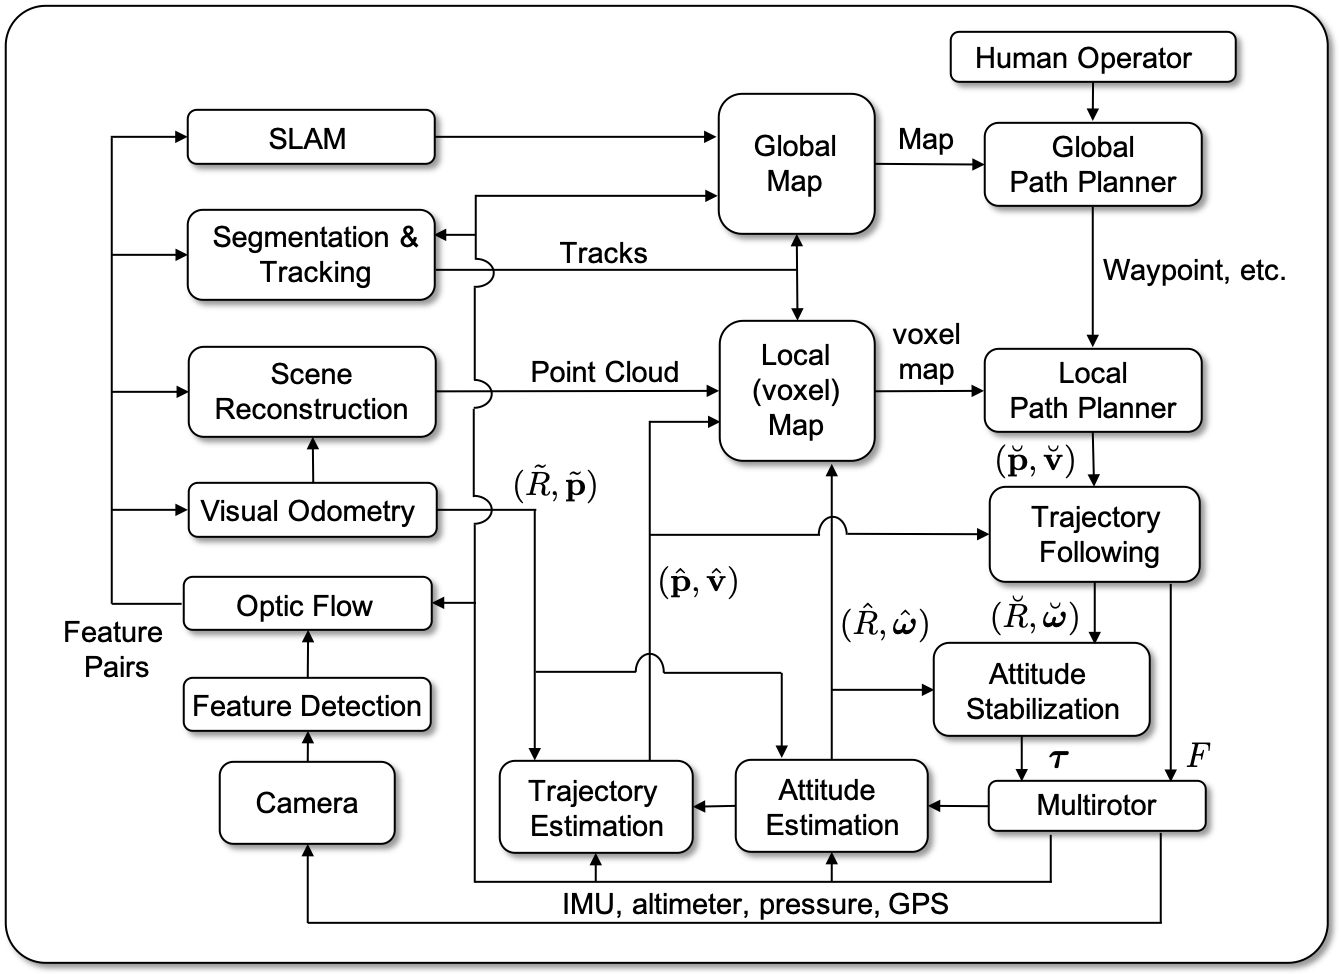
\includegraphics[width=\linewidth]{chap1_intro/figures/architecture} 
   \caption{Software architecture for multirotor estimation and control.}
   \label{fig:intro_architecture}
\end{figure*}

In the bottom right corner is the {\em Multirotor} block representing both the physical flying vehicle and the onboard sensors, including IMU, altimeter, pressure sensors, and possibly a GNSS receiver.  We also assume that the platform has a camera, which we have drawn in its own block.  The equations of motion for the multirotor and the mathematical models for the sensors will be described in Chapter~\ref{chap:multirotor}.  The commanded inputs to the multirotor will be assumed to be the force in the body $z$-axis $F$, and the torque applied to the body $\taubf$.  
%
The {\em Attitude Stabilization} block is discussed in Chapter~\ref{chap:attitude_control}.  In the literature, three different representations for attitude are commonly used, namely Euler angles, quaternions, and rotation matrices.  We will describe attitude stabilization schemes for each representation.  The output of the attitude stabilization block is the applied torque $\taubf$.  The input is the desired attitude $\breve{R}$ and the desired angular rate $\breve{\omegabf}$
%
The {\em Trajectory Following} block is discussed in Chapter~\ref{chap:trajectory_following}.  The input to the trajectory follower is the desired position $\breve{\pbf}$ and the desired velocity $\breve{\vbf}$.  

The second part of the book is concerned with cameras, computer vision, and state estimation.  The {\em Camera} and {\em Feature Detection} blocks shown in Figure~\ref{fig:intro_architecture} are described in Chaper~\ref{chap:camera_features}.  {\em Optical Flow} is discussed in Chapter~\ref{chap:optical_flow}, both how optic flow is computed, as well as how it can be used to navigate a multirotor through urban canyons.  
%
{\em Visual Odometry} is discussed in Chapter~\ref{chap:visual_odometry}.  We then return to the important task of state estimation.  {\em Attitude Estimation} is described in Chapter~\ref{chap:attitude_estimation}, where we include estimation schemes that use feature matching, optic flow, and visual odometry.  In a similar way, {\em Trajectory Estimation} is described in Chapter~\ref{chap:trajectory_estimation}. 

The final part of the book focuses on mapping and planning.  {\em Scene Reconstruction} using a {\em Local Voxel Map} is detailed in Chapter~\ref{chap:scene_reconstruction}.  {\em Segmentation and Tracking} is discussed in Chapter~\ref{chap:tracking}.  The {\em Local Path Planner} is then described in Chapter~\ref{chap:local_planner} where we describe differential flatness, spline-based planning, and visual servoing.  One particular implementation of Simultaneous Localization and Mapping ({\em SLAM}) is then described in Chapter~\ref{chap:SLAM}, and global path planning using the global map created by SLAM is described in Chapter~\ref{chap:global_planner}.






\section{Mathematical Models}

\subsection{Preliminaries}

Throughout this document, we will use bold face to denote a vector, and a superscript on the vector to denote the coordinate frame where the vector is expressed.  For example, $\mathbf{v}^r\in\mathbb{R}^3$ denotes the vector $\mathbf{v}$ expressed relative to coordinate frame $\mathcal{F}^r$.  The rotation matrix that transforms vectors expressed relative to frame $\mathcal{F}^r$ into vectors expressed relative to frame $\mathcal{F}^s$ is denoted $R_r^s\in SO(3)$.  

Let $\boldsymbol{\omega}_{r/s}$ denote the angular velocity of frame $\mathcal{F}^r$ relative to frame $\mathcal{F}^s$.  Then the kinematic equations of motion for $R_r^s$ is given by
\begin{equation}\label{eq:R_r^s}
\dot{R}_r^s = R_r^s(\boldsymbol{\omega}_{r/s}^r)^\wedge,
\end{equation}
where the {\em wedge} operator is defined as
\[
\begin{pmatrix}a \\ b \\ c\end{pmatrix}^\wedge \defeq \begin{pmatrix} 0 & -c & b \\ c & 0 & -a \\ -b & a & 0 \end{pmatrix}. 
\]
Alternatively, the {\em vee} operator is defined as
\[
\begin{pmatrix} 0 & -c & b \\ c & 0 & -a \\ -b & a & 0 \end{pmatrix}^\vee \defeq \begin{pmatrix}a \\ b \\ c\end{pmatrix}. 
\]

Recall that the cross product is invariant under rotation, or in other words
\[
R(\mathbf{v}\times\mathbf{w}) = (R\mathbf{v})\times(R\mathbf{w}),
\]
when $R\in SO(3)$.
Therefore
\begin{align*}
(R\mathbf{v})^\wedge\mathbf{w} &= (R\mathbf{v})\times \mathbf{w} \\
&= R\left(\mathbf{v}\times (R^\top \mathbf{w})\right) \\
&= R\mathbf{v}^\wedge R^\top \mathbf{w},
\end{align*}
which implies that
\begin{equation}\label{eq:Rv^wedge}
(R\mathbf{v})^\wedge = R\mathbf{v}^\wedge R^\top.
\end{equation}
Noting that $\boldsymbol{\omega}_{r/s}^s = R_r^s\boldsymbol{\omega}_{r/s}^r$, then from Equations~\eqref{eq:R_r^s} and~\eqref{eq:Rv^wedge} we have that
\begin{align*}
\dot{R}_r^s &= R_r^s(R_r^s\boldsymbol{\omega}_{r/s}^s)^\wedge \\
&= R_r^s((R_r^s)^\top\boldsymbol{\omega}_{r/s}^s)^\wedge \\
&= R_r^s (R_r^s)^\top (\boldsymbol{\omega}_{r/s}^s)^\wedge R_r^s \\
&= (\boldsymbol{\omega}_{r/s}^s)^\wedge R_r^s \\
\end{align*}

The Frobenius norm of matrix $A\in\mathbb{R}^{n\times n}$ is defined as
\[
\norm{A} \defeq \sqrt{tr[A^\top A]},
\]
where $tr(M)$ is the trace of $M$.  We will have need of the following properties of the trace:
\begin{description}
\item{T.1.} $tr\left[ A^\top \right]=tr\left[ A \right]$,
\item{T.2.} $tr\left[ AB \right] = tr\left[ BA \right]$,
\item{T.3.} $tr\left[ \alpha A + \beta B \right] = \alpha tr\left[ A \right] + \beta tr\left[ B \right]$ where $\alpha$ and $\beta$ are scalars, 
\item{T.4.} $tr\left[ AB \right] = 0$ when $A$ is a symmetric matrix and $B$ is a skew-symmetric matrix,
\item{T.5.} $tr\left[ a^\wedge b^\wedge \right] = -2a^\top b$, where $a, b \in \mathbb{R}^3$.
\end{description}

When $\tilde{R}\in SO(3)$, properties T.1 and T.3 imply that if $V\defeq \frac{1}{2}\norm{I-\tilde{R}}^2$, then
\begin{align*}
V   &= \frac{1}{2} \norm{I-\tilde{R}}^2 \\
	&= \frac{1}{2} tr\left[(I-\tilde{R})^\top(I-\tilde{R})\right] \\
  	&= \frac{1}{2} tr\left[ I - \tilde{R} - \tilde{R}^\top + \tilde{R}^\top\tilde{R}\right] \\
  	&= tr\left[I-\tilde{R}\right].
\end{align*}
Furthermore, if $\tilde{R}=\breve{R} R^\top$, where $\breve{R}, R\in SO(3)$ and 
\begin{align*}
\dot{R} &= \boldsymbol{\omega}^\wedge R \\	
\dot{\breve{R}} &=  \breve{\boldsymbol{\omega}}^\wedge \breve{R},
\end{align*}
then
\begin{align}
\dot{V} &= -tr\left[ \dot{\tilde{R}} \right] \notag \\
        &= -tr\left[ \dot{\breve{R}} R^\top + \breve{R} \dot{R}^\top \right] \notag\\
        &= -tr\left[ \breve{\boldsymbol{\omega}}^\wedge \breve{R} R^\top + \breve{R} R^\top (\boldsymbol{\omega}^\top)^\wedge \right] \notag\\
        &= -tr\left[ \breve{\boldsymbol{\omega}}^\wedge \tilde{R} - \tilde{R} \boldsymbol{\omega}^\wedge \right]. \label{eq:lyapunov_derivative_1}
\end{align}
Define the symetric and skew-symmetric operators as
\begin{align*}
\mathbb{P}_s (A) &\defeq \frac{1}{2}(A+A^\top) \\
\mathbb{P}_a (A) &\defeq \frac{1}{2}(A-A^\top),
\end{align*}
and note that $A=\mathbb{P}_s(A)+\mathbb{P}_a(A)$.  Equation \eqref{eq:lyapunov_derivative_1} then become
\begin{align}
\dot{V} &= -tr\left[ \breve{\boldsymbol{\omega}}^\wedge (\mathbb{P}_s(\tilde{R})-\mathbb{P}_a(\tilde{R})) + (\mathbb{P}_s(\tilde{R})+\mathbb{P}_a(\tilde{R})) \boldsymbol{\omega}^\wedge \right] \notag\\
&= -tr\left[ \breve{\boldsymbol{\omega}}^\wedge \mathbb{P}_a(\tilde{R}) - \mathbb{P}_a(\tilde{R}) \boldsymbol{\omega}^\wedge \right] \notag\\
&= -tr\left[  \mathbb{P}_a(\tilde{R})(\boldsymbol{\omega}-\breve{\boldsymbol{\omega}})^\wedge \right] \label{eq:lyapunov_derivative_2}
\end{align}
where the second line follows from property T.4, and the third line follows from property T.2.




\subsection{Equations of Motion}


Let $\mathbf{p}_{b/i}^i$ denote the position of the vehicle/UAV with respect to the inertial frame, as expressed in inertial coordinate, and let $\mathbf{v}_{b/i}^i$ denote the velocity of the UAV with respect to the inertial frame, expressed in inertial coordinates.  Then the translational kinematics are given by
\[
\dot{\mathbf{p}}_{b/i}^i = \mathbf{v}_{b/i}^i.
\]
Let $R_b^i\in SO(3)$ denote the rotation matrix from body coordinates to inertial coordinates, and let $\boldsymbol{\omega}_{b/i}^b$ denote the angular velocity of the UAV with respect to inertial coordinates, expressed in the body frame of the UAV.  Then the rotational kinematics are given by
\[
\dot{R}_b^i = R_b^i \left(\boldsymbol{\omega}_{b/i}^b\right)^\wedge.
\]


Let $m$ and $J$ denote the mass and inertia of the vehicle respectively, $g$ the gravitational force exerted on a unit mass at sea level, $T\in\mathbb{R}^+$ the total thrust on the UAV, $\mathbf{f}_{\text{drag}}$ the drag force on the vehicle, and $M\in\mathbb{R}^3$ the applied moments, then Newton's law implies the following dynamic equations of motion:
\begin{align*}
m\dot{\mathbf{v}}_{b/i}^i &= mg\mathbf{e}_3^i + \mathbf{f}_{\text{drag}}^i + TR_b^i\mathbf{e}_3^b \\
J\dot{\boldsymbol{\omega}}_{b/i}^b &= -\boldsymbol{\omega}_{b/i}^b \times J\boldsymbol{\omega}_{b/i}^b + \mathbf{M}^b,	
\end{align*}
where $\mathbf{e}_i^\ast$ is the three dimensional column vector with one in the $i^{th}$ row and zero in the other elements, and the superscript is added to emphasize the frame in which the unit vector is defined.  Note that $mg\mathbf{e}_3^i$ is the gravity term that is fixed in the inertial frame and points towards the center of the earth, and that $TR_b^i\mathbf{e}_3^b$ is the thrust vector that is fixed in the UAV body frame.

As shown in~\cite{LeishmanMacDonaldBeard14}, the drag term is most easily described in the multirotor body frame as 
\[
\mathbf{f}_{\text{drag}}^b = \mu \Pi_{\mathbf{e}_3}\mathbf{v}_{b/i}^b,
\]
where $\mu$ is the drag coefficient and 
\[
\Pi_\mathbf{x} \defeq I-\mathbf{x}\mathbf{x}^\top,
\]
is the projection matrix onto the two dimensional subspace that is orthogonal to the unit vector $\mathbf{x}\in\mathbb{R}^3$.  Therefore, the drag force always acts orthogonal to the thrust vector and is contained in the body fixed plane $x-y$ plane of the multirotor.  The drag force in inertial coordinates is given by
\[
\mathbf{f}_{\text{drag}}^i = \mu R_b^i\Pi_{\mathbf{e}_3}(R_b^i)^\top \mathbf{v}_{b/i}^i.  
\]

We will assume in this paper that the camera is mounted on a gimbal and that the center of the camera and gimbal frame are both located at the center of the UAV body frame, which coincides with its center of mass.  Let $\boldsymbol{\ell}_o$ denote the unit vector that is aligned with the optical axis of the camera, and let $R_c^b\in SO(3)$ denote the rotation matrix from the camera frame to the body frame.  Then the optical axis in the body frame is given by 
\[
\boldsymbol{\ell}_o^b = R_c^b \mathbf{e}_3^c.  
\]
We will assume the ability to command the angular rates of the gimbal with respect to the body.  Therefore, the kinematics of the gimbal are given by
\[
\dot{R}_c^b = R_c^b\left(\boldsymbol{\omega}_{c/b}^c\right)^\wedge
\]
where $\boldsymbol{\omega}_{c/b}^c$ are the commanded angular rates of the gimbal.

In summary, the equations of motion for the multirotor with gimbal are given by
\begin{align}
	\dot{\mathbf{p}}_{b/i}^i &= \mathbf{v}_{b/i}^i \label{eq:eom_p_b/i^i}\\
	m\dot{\mathbf{v}}_{b/i}^i &= mg\mathbf{e}_3^i + \mu R_b^i\Pi_{\mathbf{e}_3}(R_b^i)^\top \mathbf{v}_{b/i}^i + TR_b^i\mathbf{e}_3^b \label{eq:eom_v_b/i^i}\\
	\dot{R}_b^i &= R_b^i \left(\boldsymbol{\omega}_{b/i}^b\right)^\wedge \\
	J\dot{\boldsymbol{\omega}}_{b/i}^b &= -\boldsymbol{\omega}_{b/i}^b \times J\boldsymbol{\omega}_{b/i}^b + \mathbf{M}^b \\
	\dot{R}_c^b &= R_c^b\left(\boldsymbol{\omega}_{c/b}^c\right)^\wedge.
\end{align}

Note that if the UAV velocity vector is expressed in body coordinates, then the translational equations of motion become
\begin{align*}
	\dot{\mathbf{p}}_{b/i}^i &= R_b^i\mathbf{v}_{b/i}^b \\
	m\dot{\mathbf{v}}_{b/i}^b &= -\boldsymbol{\omega}_{b/i}^b\times\mathbf{v}_{b/i}^b + mg(R_b^i)^\top\mathbf{e}_3^i + \mu \Pi_{\mathbf{e}_3} \mathbf{v}_{b/i}^b + T\mathbf{e}_3^b.
\end{align*}

Let $\mathbf{p}_{t/i}\in\mathbb{R}^3$ and $\mathbf{v}_{t/i}\in\mathbb{R}^3$ be the position and velocity of the target relative to the inertial frame.  We will assume a constant velocity model where
\begin{align*}
	\dot{\mathbf{p}}_{t/i}^i &= \mathbf{v}_{t/i}^i \\
	\dot{\mathbf{v}}_{t/i}^i &= 0.	
\end{align*}
The camera measures the normalized line-of-sight vector in camera coordinate
\[
\boldsymbol{\ell}_{t/c}^c = \frac{\mathbf{p}_{t/i}^c-\mathbf{p}_{b/i}^c}{\norm{\mathbf{p}_{t/i}-\mathbf{p}_{b/i}}}
\]


\section{The Body-Level Frame}

The target-following problem will be cast in the body-level frame.  The basic idea is that the body-level frame is the un-rolled and un-pitched body frame.  The heading direction for the body frame and the body-level frame will be identical, but the $z$-axis of the body level frame will always point down along the gravity vector.
Letting $\ell$ denote the body-level frame, we have that
\[
R_b^i = R_\ell^i R_b^\ell,
\]
or 
\[
R_\ell^i =  R_b^i (R_b^\ell)^\top.
\]
To make things concrete, if $\phi$, $\theta$, and $\psi$ are the roll, pitch, and yaw Euler angles, then 
\begin{align*}
R_b^i &= R_z(\psi) R_y(\theta) R_x(\phi) \\
	&\defeq \begin{pmatrix} \cos\psi & -\sin\psi & 0 \\ \sin\psi & \cos\psi & 0 \\ 0 & 0 & 1 \end{pmatrix}
	\begin{pmatrix} \cos\theta & 0 & \sin\theta \\ 0 & 1 & 0 \\ -\sin\theta & 0 & \cos\theta \end{pmatrix}
	\begin{pmatrix} 1 & 0 & 0 \\ 0 & \cos\phi & -\sin\phi \\ 0 & \sin\phi & \cos\phi \end{pmatrix}.
\end{align*}
In this case $R_\ell^i = R_z(\psi)$ and $R_b^\ell = R_y(\theta)R_x(\phi)$.


%----------------------------------------------
\subsection{Equations of Motion of the Body-Level Frame}

Since the origin of the body-level frame is coincident with the origin of the body frame, we have that
\begin{align*}
\mathbf{p}_{\ell/i} &= \mathbf{p}_{b/i} \\	
\mathbf{v}_{\ell/i} &= \mathbf{v}_{b/i}.
\end{align*}
Therefore, using Equation~\eqref{eq:eom_p_b/i^i} and~\eqref{eq:eom_v_b/i^i} we get that the translational equations of motion in the body-level frame are given by
\begin{align*}
	\dot{\mathbf{p}}_{\ell/i}^i &= \mathbf{v}_{\ell/i}^i\\
	m\dot{\mathbf{v}}_{\ell/i}^i &= mg\mathbf{e}_3^i + \mu R_\ell^i R_b^\ell \Pi_{\mathbf{e}_3}(R_b^\ell)^\top (R_\ell^i)^\top \mathbf{v}_{\ell/i}^i + TR_\ell^i R_b^\ell \mathbf{e}_3^b.
\end{align*}

The angular velocity of the body, resolved in the body-level frame, is given by
\[
\boldsymbol{\omega}_{b/i}^\ell = R_b^\ell \boldsymbol{\omega}_{b/i}^b.
\]
Since the body-level frame only rotates about its own $\mathbf{e}_3$-axis, we have that
\begin{equation}\label{eq:omega_l/i^l}
\boldsymbol{\omega}_{\ell/i}^\ell 
	= \mathbf{e}_3 \mathbf{e}_3^\top \boldsymbol{\omega}_{b/i}^\ell
	= \mathbf{e}_3 \mathbf{e}_3^\top R_b^\ell \boldsymbol{\omega}_{b/i}^b.
\end{equation}
From Equation~\eqref{eq:R_r^s}, the kinematic equation of motion for $R_\ell^i$ is given by
\[
\dot{R}_\ell^i = R_\ell^i(\boldsymbol{\omega}_{\ell/i}^\ell)^\wedge.
\]

Differentiating Equation~\eqref{eq:omega_l/i^l} gives
\[
\dot{\boldsymbol{\omega}}_{\ell/i}^\ell = \mathbf{e}_3\mathbf{e}_3^\top \left[ R_b^\ell \dot{\boldsymbol{\omega}}_{b/i}^b + \dot{R}_b^\ell \boldsymbol{\omega}_{b/i}^b \right].
\]
From Equation~\eqref{eq:R_r^s} we have that
\[
\dot{R}_b^\ell = R_b^\ell (\boldsymbol{\omega}_{b/\ell}^b)^\wedge,
\]
where 
\[
\boldsymbol{\omega}_{b/\ell}^b = \boldsymbol{\omega}_{b/i}^b - \boldsymbol{\omega}_{\ell/i}^b,
\]
which implies that
\begin{align*}
\dot{\boldsymbol{\omega}}_{\ell/i}^\ell &= \mathbf{e}_3\mathbf{e}_3^\top \left[ R_b^\ell \dot{\boldsymbol{\omega}}_{b/i}^b + R_b^\ell (\boldsymbol{\omega}_{b/i}^b - \boldsymbol{\omega}_{\ell/i}^b)^\wedge \boldsymbol{\omega}_{b/i}^b \right] \\
&= \mathbf{e}_3\mathbf{e}_3^\top \left[ R_b^\ell \dot{\boldsymbol{\omega}}_{b/i}^b - R_b^\ell (\boldsymbol{\omega}_{\ell/i}^b)^\wedge \boldsymbol{\omega}_{b/i}^b \right] \\
&= \mathbf{e}_3\mathbf{e}_3^\top R_b^\ell \left[  J^{-1}\mathbf{M}^b - J^{-1}(\boldsymbol{\omega}_{b/i}^b)^\wedge (J\boldsymbol{\omega}_{b/i}^b) + (\boldsymbol{\omega}_{b/i}^b)^\wedge \boldsymbol{\omega}_{\ell/i}^b \right] \\
\end{align*}

Using Equation~\eqref{eq:R_r^s} and the fact that $(Rv)^\wedge = Rv^\wedge R^\top$ we get that
\[
\dot{R}_r^s = (\boldsymbol{\omega}_{r/s}^s)^\wedge R_r^s,
\]
which implies that
\[
\dot{R}_b^\ell = (\boldsymbol{\omega}_{b/\ell}^\ell)^\wedge R_b^\ell.
\]
Using the facts that $\boldsymbol{\omega}_{b/\ell}^\ell = \boldsymbol{\omega}_{b/i}^\ell - \boldsymbol{\omega}_{\ell/i}^\ell$ and $\boldsymbol{\omega}_{b/i}^\ell = R_b^\ell \boldsymbol{\omega}_{b/i}^b$, we have that
\begin{align*}
\dot{\boldsymbol{\omega}}_{b/\ell}^\ell &= 	\dot{\boldsymbol{\omega}}_{b/i}^\ell - \dot{\boldsymbol{\omega}}_{\ell/i}^\ell \\
&= R_b^\ell \dot{\boldsymbol{\omega}}_{b/i}^b + R_b^\ell(\boldsymbol{\omega}_{b/\ell}^b)^\wedge \boldsymbol{\omega}_{b/i}^b - \dot{\boldsymbol{\omega}}_{\ell/i}^\ell \\
&= R_b^\ell\left[  J^{-1}\mathbf{M}^b - J^{-1}(\boldsymbol{\omega}_{b/i}^b)^\wedge (J\boldsymbol{\omega}_{b/i}^b) + (\boldsymbol{\omega}_{b/i}^b)^\wedge \boldsymbol{\omega}_{\ell/i}^b \right]- \dot{\boldsymbol{\omega}}_{\ell/i}^\ell \\
&= (I-\mathbf{e}_3\mathbf{e}_3^\top) R_b^\ell\left[  J^{-1}\mathbf{M}^b - J^{-1}(\boldsymbol{\omega}_{b/i}^b)^\wedge (J\boldsymbol{\omega}_{b/i}^b) + (\boldsymbol{\omega}_{b/i}^b)^\wedge \boldsymbol{\omega}_{\ell/i}^b \right].
\end{align*}

Summarizing, the dynamics in the body-level frame are given by
\begin{align}
	\dot{\mathbf{p}}_{\ell/i}^i &= \mathbf{v}_{\ell/i}^i \label{eq:pdot_l/i^i}\\
	m\dot{\mathbf{v}}_{\ell/i}^i &= mg\mathbf{e}_3^i + \mu R_\ell^i R_b^\ell \Pi_{\mathbf{e}_3}(R_b^\ell)^\top (R_\ell^i)^\top \mathbf{v}_{\ell/i}^i + TR_\ell^i R_b^\ell \mathbf{e}_3^b \label{eq:vdot_l/i^i}\\
	\dot{R}_\ell^i &= R_\ell^i(\boldsymbol{\omega}_{\ell/i}^\ell)^\wedge \label{eq:Rdot_l^i}\\
	\dot{\boldsymbol{\omega}}_{\ell/i}^\ell &=\mathbf{e}_3\mathbf{e}_3^\top R_b^\ell \left[  J^{-1}\mathbf{M}^b - J^{-1}(\boldsymbol{\omega}_{b/i}^b)^\wedge (J\boldsymbol{\omega}_{b/i}^b) + (\boldsymbol{\omega}_{b/i}^b)^\wedge \boldsymbol{\omega}_{\ell/i}^b \right] \label{eq:omegadot_l/i^l} \\
	\dot{R}_b^\ell &= R_b^\ell (\boldsymbol{\omega}_{b/\ell}^b)^\wedge  \label{eq:Rdot_b^l} \\
	\dot{\boldsymbol{\omega}}_{b/\ell}^\ell &= 	\Pi_{\mathbf{e}_3} R_b^\ell\left[  J^{-1}\mathbf{M}^b - J^{-1}(\boldsymbol{\omega}_{b/i}^b)^\wedge (J\boldsymbol{\omega}_{b/i}^b) + (\boldsymbol{\omega}_{b/i}^b)^\wedge \boldsymbol{\omega}_{\ell/i}^b \right]. \label{eq:omegadot_b/l^l}
\end{align}


%----------------------------------------------
\subsection{Feedback Projecting Control}

In this section we develop a feedback linearizing control that will facilitate tracking in the local level frame.  The first step is to let 
\[
\mathbf{M}^b = (\boldsymbol{\omega}_{b/i}^b)^\wedge(J\boldsymbol{\omega}_{b/i}^b - J(\boldsymbol{\omega}_{b/i}^b)^\wedge\boldsymbol{\omega}_{\ell/i}^b + J(R_b^\ell)^\top \begin{pmatrix}u_\phi \\ u_\theta \\ u_\psi \end{pmatrix}.
\]
Substituting into Equations~\eqref{eq:omegadot_l/i^l} and \eqref{eq:omegadot_b/l^l} gives
\begin{align*}
	\dot{\boldsymbol{\omega}}_{\ell/i}^\ell &=\mathbf{e}_3 u_\psi \\
	\dot{\boldsymbol{\omega}}_{b/\ell}^\ell &= 	\begin{bmatrix} \mathbf{e}_1 & \mathbf{e}_2 \end{bmatrix}\begin{pmatrix}u_\phi \\ u_\theta \end{pmatrix} \defeq E_{12}u_{12}.
\end{align*}

Ignoring the drag term, i.e., setting $\mu=0$, Equations~\eqref{eq:pdot_l/i^i} and~\eqref{eq:vdot_l/i^i} become
\[
\ddot{\mathbf{p}}_{\ell/i}^i = g\mathbf{e}_3 + \frac{T}{m}R_\ell^i R_b^\ell \mathbf{e}_3.
\]
Throughout the paper, we will use the "breve" mark to denote a desired quantity.  Accordingly, by selecting $\breve{\mathbf{u}}_{\ell/i}^i$ as the desired acceleration in the body level frame, $\breve{\mathbf{R}}_b^\ell\in SO(3)$ as the desired rotation from body to body-level frames, and $\breve{T}\in\mathbb{R}$ as the desired thrust, we get that
\[
\frac{\breve{T}}{m} \breve{R}_b^\ell \mathbf{e}_3 = (R_\ell^i)^\top\left(\breve{\mathbf{u}}_{\ell/i}^i - g\mathbf{e}_3\right).
\]
Letting
\[
\breve{R}_b^\ell = \begin{bmatrix} \breve{\mathbf{r}}_{1}, & \breve{\mathbf{r}}_{2}, & \breve{\mathbf{r}}_{3}\end{bmatrix}
\]
we get that 
\begin{align*}
\breve{T} &= m\norm{\breve{\mathbf{u}}_{\ell/i}^i - g\mathbf{e}_3} \\
\breve{\mathbf{r}}_{3} &= \frac{(R_\ell^i)^\top (\breve{\mathbf{u}}_{\ell/i}^i - g\mathbf{e}_3)}{\norm{\breve{\mathbf{u}}_{\ell/i}^i - g\mathbf{e}_3}}.
\end{align*}

Since $R_b^\ell$ represents only the roll and pitch angles of the body, the first column of $\breve{R}_b^\ell$ is defined so that it is in the $x-z$ plane of the local-level frame, i.e., perpendicular to $\mathbf{e}_2$ and a $90$~degree rotation of $\breve{\mathbf{r}}_{3}$.  Therefore
\[
\breve{\mathbf{r}}_{1} = \frac{R_y(\frac{\pi}{2})(I-\mathbf{e}_2\mathbf{e}_2^\top)\breve{\mathbf{r}}_{3}}{\norm{(I-\mathbf{e}_2\mathbf{e}_2^\top)\breve{\mathbf{r}}_{3}}}.
\]
The second column of $\breve{R}_b^\ell$ is selected to form a right handed coordinate system as
\[
\breve{\mathbf{r}}_{2} = \breve{\mathbf{r}}_{3} \times \breve{\mathbf{r}}_{1}.
\]

Note that since
\[
R_y(\frac{\pi}{2})(I-\mathbf{e}_2\mathbf{e}_2^\top) = \begin{pmatrix}0 & 0 & 1 \\ 0 & 1 & 0 \\ -1 & 0 & 0\end{pmatrix}\begin{pmatrix}1 & 0 & 0 \\ 0 & 0 & 0 \\ 0 & 0 & 1\end{pmatrix} = \begin{pmatrix} 0 & 0 & 1 \\ 0 & 0 & 0 \\ -1 & 0 & 0 \end{pmatrix},
\]
then if $\breve{\mathbf{r}}_{3} = (a, b, c)^\top$, then $\breve{\mathbf{r}}_{1} = (c, 0, -a)^\top/\sqrt{a^2+c^2}$, and $\breve{\mathbf{r}}_{2} = (-ab, a^2+c^2, -bc)^\top/\sqrt{a^2+c^2}$, which implies that 
\[
\breve{R}_b^\ell = \begin{pmatrix} \frac{c}{\alpha} & \frac{-ab}{\alpha} & a \\
                               0 & \alpha & b \\
                               \frac{-a}{\alpha} & \frac{-bc}{\alpha} & c
               \end{pmatrix},
\] 
where $\alpha = \sqrt{a^2+c^2}$.

Let $\dot{\breve{R}}_b^\ell$ be the time derivative of $\breve{R}_b^\ell$, which is assumed to be computed numerically.  Then since $\dot{\breve{R}}_b^\ell = (\breve{\boldsymbol{\omega}}_{b/\ell}^\ell)^\wedge\breve{R}_b^\ell$ we have that
\[
\breve{\boldsymbol{\omega}}_{b/\ell}^\ell = \left[\dot{\breve{R}}_b^\ell(\breve{R}_b^\ell)^\top \right]^\vee.
\]
Define the Lyapunov function
\begin{align*}
V &= \frac{1}{2}\norm{I-\breve{R}_b^\ell (R_b^\ell)^\top}^2 + \frac{1}{2}\norm{\boldsymbol{\omega}_{b/\ell}^\ell-\breve{\boldsymbol{\omega}}_{b/\ell}^\ell}^2 \\
  &= tr\left[I-\breve{R}_b^\ell (R_b^\ell)^\top\right]+ \frac{1}{2}\norm{\boldsymbol{\omega}_{b/\ell}^\ell-\breve{\boldsymbol{\omega}}_{b/\ell}^\ell}^2.
\end{align*}
Then from Equation~\eqref{eq:lyapunov_derivative_2}, differentiation with respect to time gives
\begin{align*}
\dot{V} &= -tr\left[  \mathbb{P}_a\left(\breve{R}_b^\ell (R_b^\ell)^\top\right)\left(\boldsymbol{\omega}_{b/\ell}^\ell-\breve{\boldsymbol{\omega}}_{b/\ell}^\ell\right)^\wedge \right] + \left(\boldsymbol{\omega}_{b/\ell}^\ell-\breve{\boldsymbol{\omega}}_{b/\ell}^\ell\right)^\top\left(\dot{\boldsymbol{\omega}}_{b/\ell}^\ell-\dot{\breve{\boldsymbol{\omega}}}_{b/\ell}^\ell\right) \\
&= 2\left(\boldsymbol{\omega}_{b/\ell}^\ell-\breve{\boldsymbol{\omega}}_{b/\ell}^\ell\right)^\top \left( \mathbb{P}_a(\breve{R}_b^\ell (R_b^\ell)^\top)\right)^\vee + \left(\boldsymbol{\omega}_{b/\ell}^\ell-\breve{\boldsymbol{\omega}}_{b/\ell}^\ell\right)^\top\left(\dot{\boldsymbol{\omega}}_{b/\ell}^\ell-\dot{\breve{\boldsymbol{\omega}}}_{b/\ell}^\ell\right) \\ 
&= \left(\boldsymbol{\omega}_{b/\ell}^\ell-\breve{\boldsymbol{\omega}}_{b/\ell}^\ell\right)^\top \left( E_{12}u_{12}-\dot{\breve{\boldsymbol{\omega}}}_{b/\ell}^\ell + 2\left( \mathbb{P}_a(\breve{R}_b^\ell (R_b^\ell)^\top)\right)^\vee \right).
\end{align*}
Therefore, select
\[
u_{12} = E_{12}^\top\left[\dot{\breve{\boldsymbol{\omega}}}_{b/\ell}^\ell - 2\left( \mathbb{P}_a(\breve{R}_b^\ell (R_b^\ell)^\top)\right)^\vee -  K_d\left(\boldsymbol{\omega}_{b/\ell}^\ell-\breve{\boldsymbol{\omega}}_{b/\ell}^\ell\right) \right],
\]
and note that $E_{12}E_{12}^\top = \Pi_{\mathbf{e}_3}$ to get
\begin{multline*}
\dot{V} = - \left(\boldsymbol{\omega}_{b/\ell}^\ell-\breve{\boldsymbol{\omega}}_{b/\ell}^\ell\right)^\top \Pi_{\mathbf{e}_3} K_d\left(\boldsymbol{\omega}_{b/\ell}^\ell-\breve{\boldsymbol{\omega}}_{b/\ell}^\ell\right) \\
   + \left(\boldsymbol{\omega}_{b/\ell}^\ell-\breve{\boldsymbol{\omega}}_{b/\ell}^\ell\right)^\top \mathbf{e}_3\mathbf{e}_3^\top \left(\dot{\breve{\boldsymbol{\omega}}}_{b/\ell}^\ell - 2\left( \mathbb{P}_a(\breve{R}_b^\ell (R_b^\ell)^\top)\right)^\vee\right).
\end{multline*}

\rwbcomment{Need to show that second term on RHS is zero}

\rwbcomment{Need to revise the stuff below to include $\Pi_{e_3}$.}

Define $\tilde{R} = \breve{R}_b^\ell (R_b^\ell)^\top$ and $\tilde{\boldsymbol{\omega}}=\boldsymbol{\omega}_{b/\ell}^\ell-\breve{\boldsymbol{\omega}}_{b/\ell}^\ell$, 
and define $E=\{(\tilde{R},\tilde{\boldsymbol{\omega}}) | \tilde{\boldsymbol{\omega}}=0\}$, 
and let $M$ be the largest invariant set in $E$. Then for all trajectories in $M$ we have that
\[
\frac{d}{dt}\norm{I-\tilde{R}}^2 = -tr\left[\mathbb{P}_a(\tilde{R})\tilde{\boldsymbol{\omega}}^\wedge\right] \equiv 0,
\]
which implies that $\tilde{R}$ is a constant matrix.  
Therefore for all trajectories in $M$
\begin{align*}
& \dot{\tilde{R}} = \tilde{R}(\boldsymbol{\omega}_{b/\ell}^b)^\wedge - (\breve{\boldsymbol{\omega}}_{b/\ell}^b)^\wedge \tilde{R} = 0 \\
\implies & \tilde{R}(\boldsymbol{\omega}_{b/\ell}^b)^\wedge = (\breve{\boldsymbol{\omega}}_{b/\ell}^b)^\wedge \tilde{R} \\
\implies & \tilde{R}(\boldsymbol{\omega}_{b/\ell}^b)^\wedge \tilde{R}^\top = (\breve{\boldsymbol{\omega}}_{b/\ell}^b)^\wedge  \\
\implies & (\tilde{R}\boldsymbol{\omega}_{b/\ell}^b)^\wedge = (\breve{\boldsymbol{\omega}}_{b/\ell}^b)^\wedge  \\
\implies & \tilde{R}\boldsymbol{\omega}_{b/\ell}^b = \breve{\boldsymbol{\omega}}_{b/\ell}^b,
\end{align*}
but since $\boldsymbol{\omega}_{b/\ell}^b=\breve{\boldsymbol{\omega}}_{b/\ell}^b$ on $M$, it must be that $\tilde{R}=I$ on $M$.  
Therefore, by the LaSalle invariance principle, $R_b^\ell \to \breve{R}_b^\ell$ and $\boldsymbol{\omega}_{b/\ell}^b\to\breve{\boldsymbol{\omega}}_{b/\ell}^b$.












\rwbcomment{The goal is to simplify the dynamics to the following:
\begin{align*}
\ddot{\mathbf{p}}_{\ell/i}^i &= \mathbf{u}_{\ell/i}^i \\
\dot{R}_\ell^i &= R_\ell^i(\boldsymbol{\omega}_{\ell/i}^\ell)^\wedge \\
\dot{\boldsymbol{\omega}}_{\ell/i}^\ell &= \mathbf{e}_3 u_\psi.
\end{align*}

}


\section{Target Following in 2D}

We begin with the simplified scenario of following a target in a two-dimensional world.  The following scenario is shown in Figure~\ref{fig:following_2d}.
\begin{figure}[hbt]
  \centering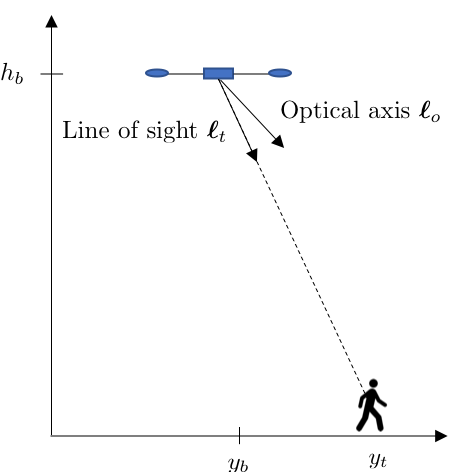
\includegraphics[width=0.5\textwidth]{./figures/following_2d}
  \caption{The following scenario in two dimensions.}
  \label{fig:following_2d}
\end{figure}

We will assume in this section that the body-level dynamics of the camera are given by
\begin{align*}
\ddot{y}_b &= u_1 \\
\ddot{h}_b &= u_2,	
\end{align*}
where the height above ground $h_b$ is in general unknown.  We assume that the optical axis $\boldsymbol{\ell}_o$ is fixed in the body level frame, and that the camera measures 
\[
\boldsymbol{\ell}_t = \frac{\mathbf{p}_{t/\ell}}{\norm{\mathbf{p}_{t/\ell}}}
\]
where
$\mathbf{p}_{t/\ell}= \begin{pmatrix} y_t-y_b, -h_b \end{pmatrix}^\top$.  
The controller also has access to $\dot{\boldsymbol{\ell}}_t$ and $\ddot{\boldsymbol{\ell}}_t$ by numerically differentiating $\boldsymbol{\ell}_t$.  



use "body-level" frame $\mathbf{p}_{\ell/i}$


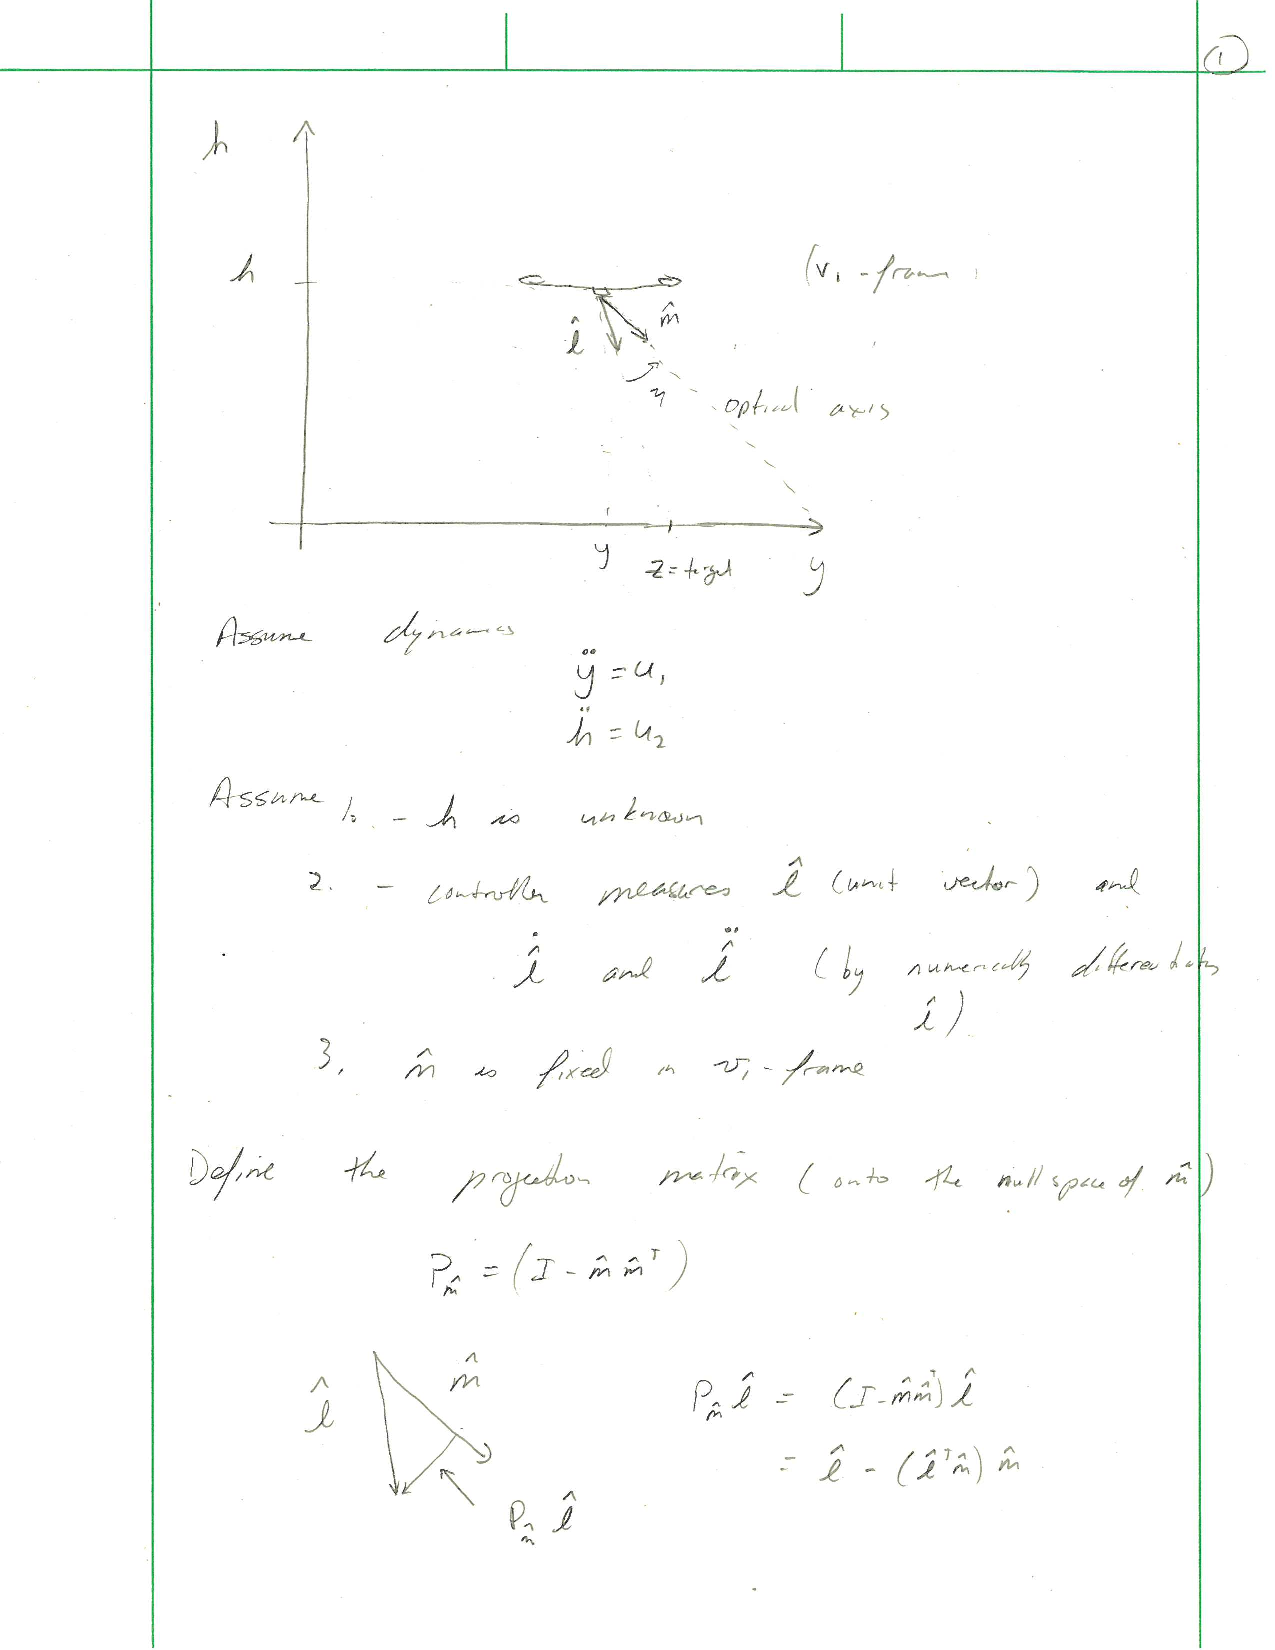
\includepdf[pages=-,scale=.8,pagecommand={}]{adaptive_following_controller.pdf}

\section{Conclusion}




\section*{Acknowledgments}
Funded by...

\bibliographystyle{IEEEtran}
\bibliography{../bib/library}

\end{document}


1